\chapter{Implemented Solution}
\section{Amazon Web Services}

\subsection{Architecture}
Since Amazon Elastic Beanstalk (EB) has been used as the core component to manage the system, it has been possibile to use an Infrastructure as a Service grade of customization, with an easier configuration and building phase as if the system were Platform as a Service instead.\\
As shown in the picture \ref{fig:architecture}, everything but the SES service is hosted in the eu-central-1 region in Frankfurt, to reduce latency, minimize costs and keep healthcare data in an European law venue, as in production would be.
EB 

\begin{figure}[h]
    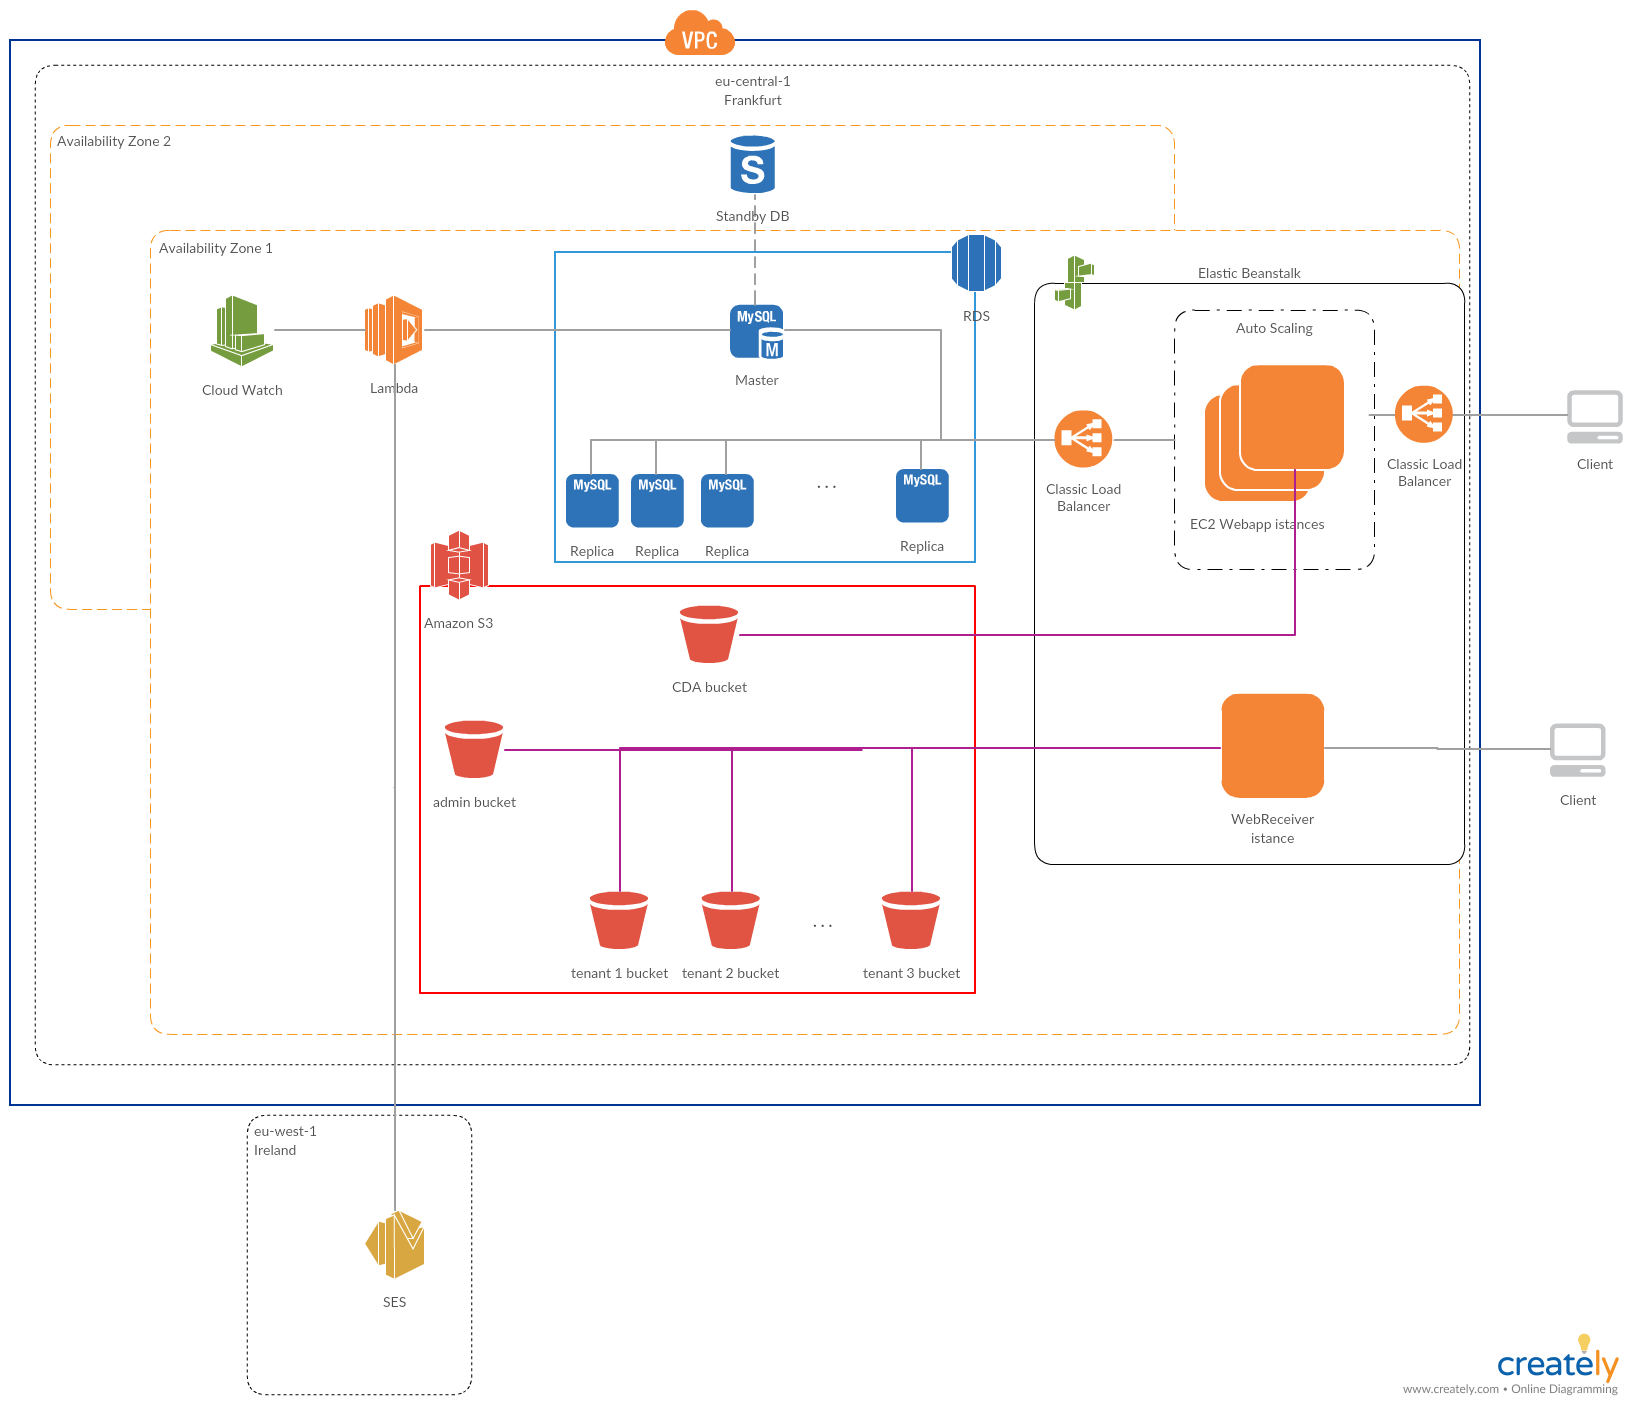
\includegraphics[width=\textwidth]{architecture}
    \caption{Architecture Scheme}
    \label{fig:architecture}
\end{figure}
\section{Ecg Workflow}
\begin{figure}[h]
    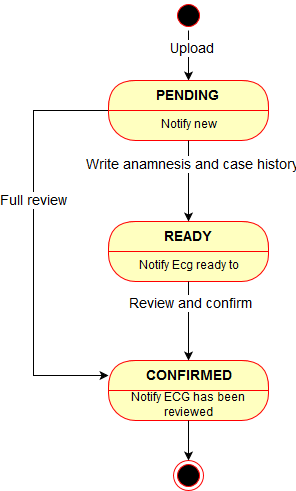
\includegraphics[width=8cm]{ECGstatechart}
    \caption{Electrocardiogram State Chart}
    \label{fig:ECGstatechart}
\end{figure}
\section{Notification}
\section{Interoperability of digital electrocardiograms data}
\subsection{Resting}
\subsection{Cardiac stress test}
\subsection{Holter}
\paragraph{Web Receiver}
\paragraph{Web Uploader}
\paragraph{S3 Bucket synchronization}